\chapter{Convolution Demonstration}
% Authors: Mimee Xu , Sai Anirudh Kondaveeti, Rui Jiang(rj1407), 2/20/18.
\s
\section{Natural Signal Patterns}

Stationarity - The waveform heights of audio signals form a sinusoidal pattern with similar
sub-segments of peaks and valleys occurring repeatedly throughout the signal.

Locality - The correlation is high between two peaks in the waveform at nearby points in time, but the correlation is low between distant peaks. Sounds have “local” properties such as being more transient or smoother in the time-frequency domain [Espi et al.]. If an audio signal were shuffled, so that the index of the data no longer represented a position in time, the audio signal would no
longer adhere to the stationarity and locality assumptions.



\section{Audio Example}
Here, we use a python library "librosa", which is for audio and music analysis. Select natural signal: \begin{verbatim}audio.wav\end{verbatim}

%% Insert wave form here
\begin{figure}[ht]
    \centering
    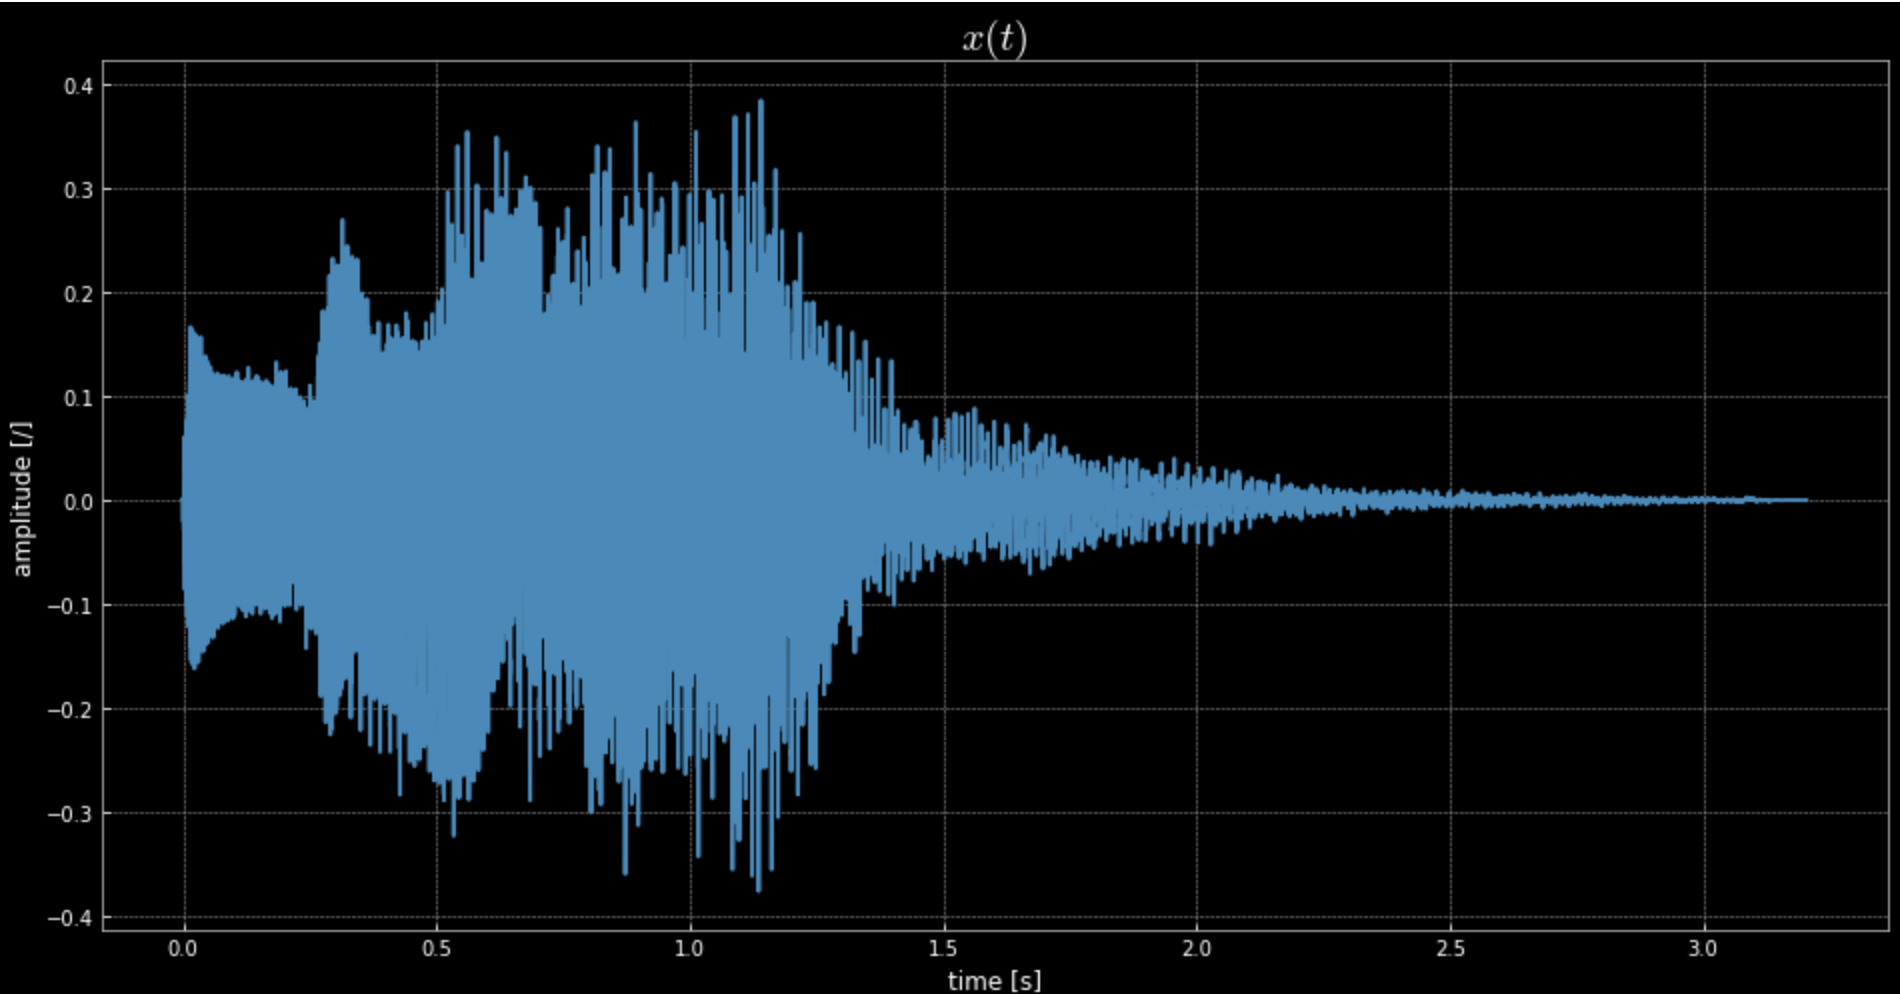
\includegraphics[width=300pt]{labs/04/images/1.png}
    \label{fig:waveform}
\end{figure}

The wave form constitutes of the magnitudes aka. volume in the time domain. To analyze it in the frequency domain where pitch can be seen and potentially separated, we use discrete Fourier Transform to obtain the Fourier Transform over every windowed signal. The resulting graph is called a spectrogram, which represents the signal in the frequency domain.

%% Insert two spectrograms here
\begin{figure}[ht]
    \centering
    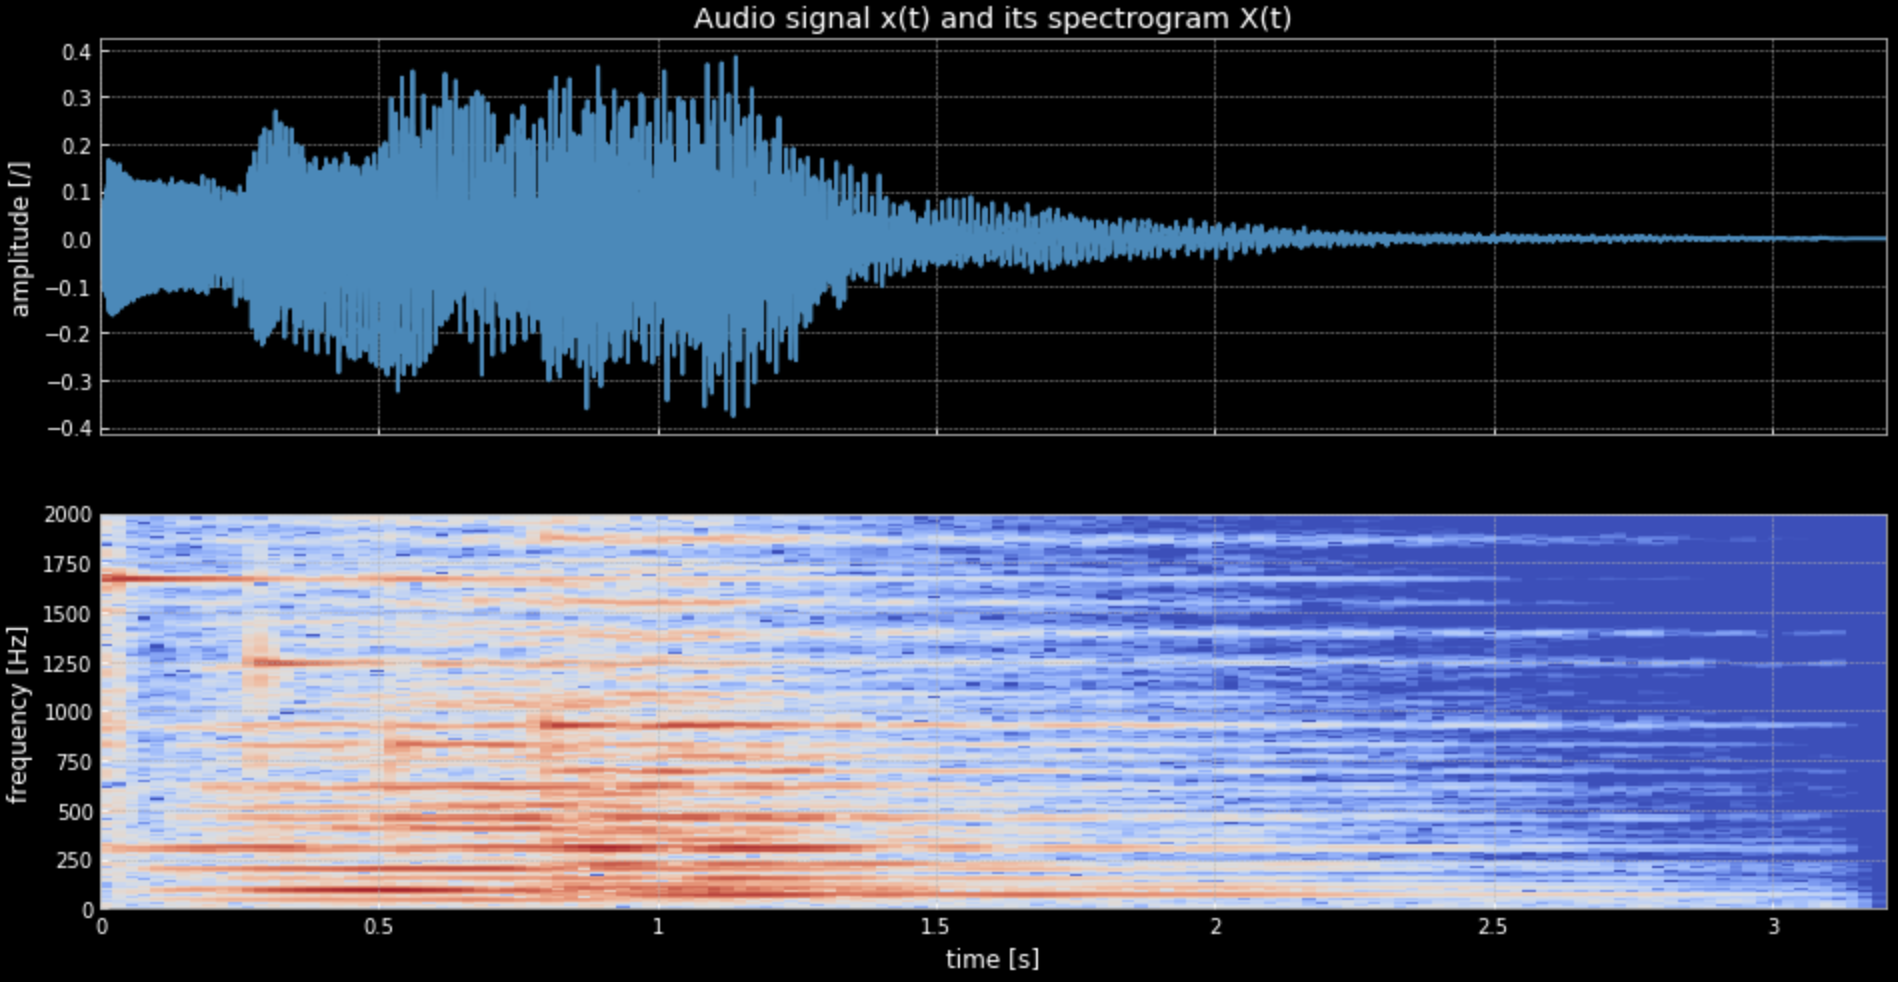
\includegraphics[width=300pt]{labs/04/images/2.png}
    \label{fig:spectrogram}
\end{figure}

The challenge is to figure out which corresponding piano keys we should play to reproduce the audio.

Then we manually reconstruct of the melody using the melody frequencies/notes from the spectrogram above and compute the Short-time Fourier transform of the reconstruction. Plot it with the original together:
%% insert two spectrograms of orginal and reconstruction
\begin{figure}[ht]
    \centering
    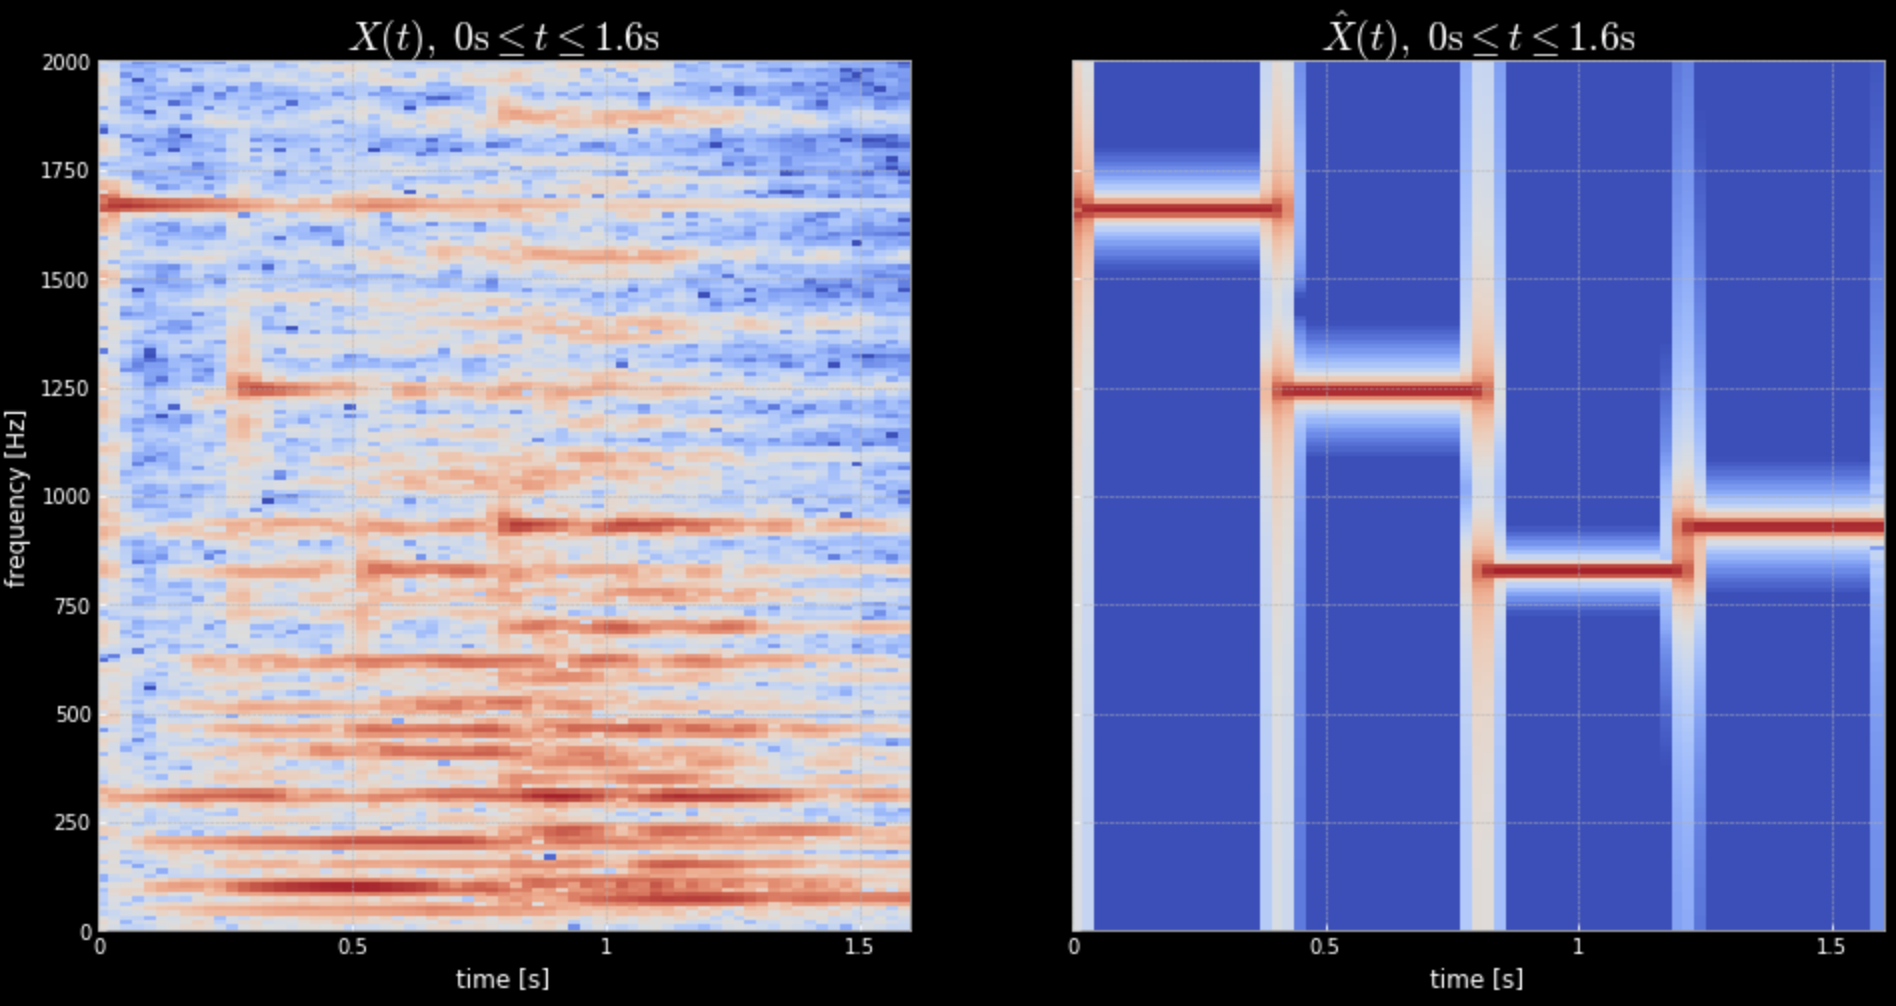
\includegraphics[width=300pt]{labs/04/images/3.png}
    \label{fig:spectrograms of original and reconstruction}
\end{figure}
